\documentclass[16 pt]{amsart}
\usepackage{amscd,amsmath,amsthm,amssymb}
\usepackage{enumerate,varioref}
\usepackage{epsfig}
\usepackage{graphicx}
\usepackage{mathtools}
\usepackage{tikz}
\usepackage{amsfonts}
\usepackage{svg}
\usetikzlibrary{graphs,arrows,topaths}
\newtheorem{thm}{Theorem}
\newtheorem{cor}[thm]{Corollary}
\newtheorem{lem}[thm]{Lemma}
\newtheorem{prop}[thm]{Proposition}
\theoremstyle{definition}
\newtheorem{defn}[thm]{Definition}
\theoremstyle{remark}
\newtheorem{ex}[thm]{Example}
\newtheorem{rem}[thm]{Remark}
\numberwithin{equation}{subsection}
\newcommand{\R}{\mathbb{R}}
\newcommand{\Z}{\mathbb{Z}}
\newcommand{\C}{\mathbb{C}}
\newcommand{\Q}{\mathbb{Q}}
\newcommand{\trail}[3]{a e_{#1} b e_{#2} a e_{#3} b e_5 c }
\begin{document}

\title{Homework 4 Maths 140 Winter 2015}
\maketitle 


10.1.22: Find a simple graph with five vertices of degrees 2,3,3,3,5

\vspace{1in}

Solution: A simple graph may not have any parallel edges or loops.  Since there are five vertices, the maximum degree any single vertex can have in a simple graph is 4.  Thus including a vertex with degree 5 makes this graph fail to be simple.


\newpage



10.1.33: Recall $K_n$ denotes a complete graph on $n$ vertices. 

a. Draw $K_6$

\vspace{.5in}

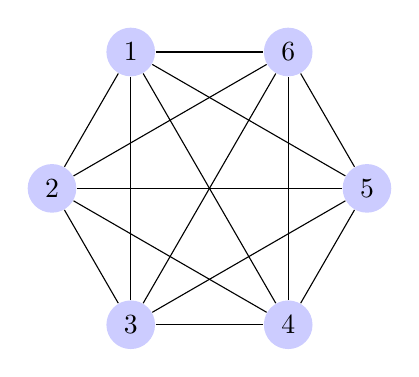
\begin{tikzpicture}
 [scale=2,auto=left,every node/.style={circle,fill=blue!20}]
 \foreach \name/\angle in {5/0,6/60,1/120,2/180,3/240,4/300}
 \node (\name) at (\angle:1) {$\name$};
 \foreach \from/\to in {1/2,1/3,1/4,1/5,1/6,2/3,2/4,2/5,2/6,3/4,3/5,3/6,4/5,4/6,5/6}
  \draw  (\from) -- (\to);
\end{tikzpicture}






\vspace{.5in}


b. Show that for $n>0, |E(K_n)| = \frac{n(n-1)}{2}$

\vspace{.5in}

Solution:  Each of the $n$ vertices connects to every other vertex with exactly one edge.  That is to say the degree of each vertex is $n-1$ And the total degree of the graph
\[
deg(K_n) = (n-1)+\cdots +(n-1) = n(n-1) = 2 |E(K_n)|.
\]


So using the handshake theorem and the degree of $K_n$ we see
\[
|E(K_n)| = \frac{n(n-1)}{2}
\]

\newpage



10.2.5: Consider the following graph:

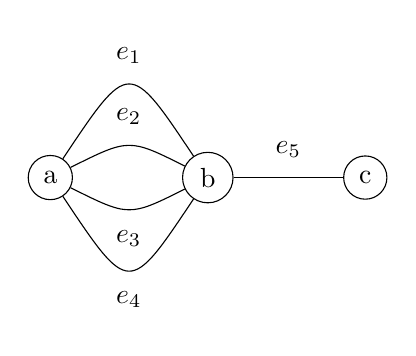
\begin{tikzpicture}
[scale=2,auto=left,every node/.style={circle}]
\node[circle,draw] (a) at (0,0){a};
\node[circle,draw] (b) at (1,0){b};
\node[circle,draw] (c) at (2,0){c};
\draw (a)..controls(.5,.25).. (b)node[midway,above]{$e_2$};
\draw (a)..controls(.5,-.25)..(b)node[midway,below]{$e_3$};
\draw (a)..controls(.5,.75)..(b)node[midway,above]{$e_1$};
\draw (a)..controls(.5,-.75)..(b)node[midway,below]{$e_4$};
\draw (b) -- (c) node[midway, above] {$e_5$};;
\end{tikzpicture}


a. How many paths from a to c?

\vspace{.5in}

Solution: Recalling that a path may not repeat vertices we have only the walks which take the form $a e_{i} b e_5 c$ where $i$ runs from 1 to 4.  Thus there are four trails.

\vspace{.5in}

b. How many trails from a to c? 

\vspace{.5in}

Solution: With trails we are not allowed to repeat edges, but repeated vertices are allowed.  In particular, all paths are trails, but not the other way around.  So in addition to our frou paths from above, we have 4 edges from $a$ to $b$.  After we have used one of these edges we have 3 edges left to return from $b$ to $a$.  Then there are 2 edges to make the final trip from $a$ to $b$ and then only one to go to $c$.  Which leaves us with $4\cdot 3\cdot 2\cdot 1= 24$ trails which are not paths (4+24 =28 overall).

Excplicitly:
\begin{eqnarray*}
\trail{1}{2}{3}, & \trail{1}{2}{4},\\
\trail{1}{3}{2}, & \trail{1}{3}{4},\\
\trail{1}{4}{2}, & \trail{1}{4}{3},\\
\trail{2}{1}{3}, & \trail{2}{1}{4},\\
\trail{2}{3}{1}, & \trail{2}{3}{4},\\
\trail{2}{4}{1}, & \trail{2}{4}{3},\\
\trail{3}{1}{2}, & \trail{3}{1}{4},\\
\trail{3}{2}{1}, & \trail{3}{2}{4},\\
\trail{3}{4}{1}, & \trail{3}{4}{2},\\
\trail{4}{1}{2}, & \trail{4}{1}{3},\\
\trail{4}{2}{1}, & \trail{4}{2}{3},\\
\trail{4}{3}{1}, & \trail{4}{3}{2}.
\end{eqnarray*}


\vspace{.5in}

c. How many walks from a to c?

\vspace{.5in}

Solution: Since there is no restriction on repeating edges or vertices for walks, we can shuttle back and forth between vertices $a$ and $b$ indefinitely and thus there are infinitely many walks from $a$ to $c$.

Let's prove this by contradiction.\\
Suppose there were a finite number of walks from $a$ to $c$.  Let's say the longest one has length $n<\infty$ and call it $W_{max}$.  Then consider the walk
\[
W_{max}e_5 b e_5 c.
\]
This new walk is a walk from $a$ to $c$ but has length $n+2$ which contradicts $n$'s being the longest walk. Therefore there are infinitely many walks from $a$ to $c$.

\newpage

10.2.32: Give two examples of graphs which have Euler circuits, but not Hamilton circuits

\vspace{1in}

Solution: In this case we need a graph that ``pinches."  The bowtie graph or a graph connecting two sqaures at a point will suffice.

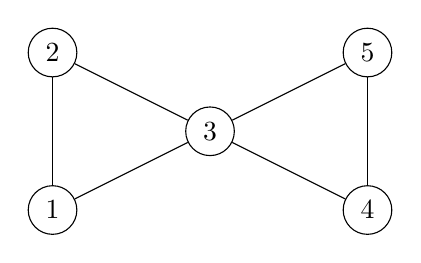
\begin{tikzpicture}
\node[circle,draw] (1) at (0,0){1};
\node[circle,draw] (2) at (0,2){2};
\node[circle,draw] (3) at (2,1){3};
\node[circle,draw] (4) at (4,0){4};
\node[circle,draw] (5) at (4,2){5};
\foreach \from/\to in {1/2,1/3,2/3,3/5,3/4,4/5}
  \draw (\from) -- (\to);
\end{tikzpicture}

\vspace{.5in}


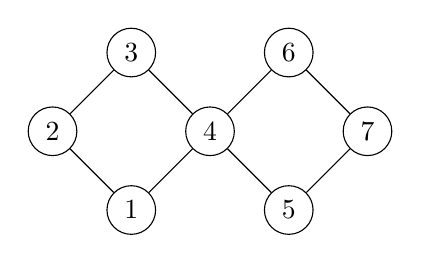
\begin{tikzpicture}
\node[circle,draw] (1) at (0,0){1};
\node[circle,draw] (2) at (-1,1){2};
\node[circle,draw] (3) at (0,2){3};
\node[circle,draw] (4) at (1,1){4};
\node[circle,draw] (5) at (2,0){5};
\node[circle,draw] (6) at (2,2){6};
\node[circle,draw] (7) at (3,1){7};
\foreach \from/\to in {1/2,1/4,2/3,7/5,6/7,3/4,4/6,4/5}
  \draw (\from) -- (\to);
\end{tikzpicture}




\newpage

10.2.33: Give two examples of graphs that have both Euler and Hamilton circuits.

\vspace{1in}

Solution: Here we can use any complete graph on an odd number of vertices. Or any polygonal graph with an edge of odd degree:

\vspace{.5in}

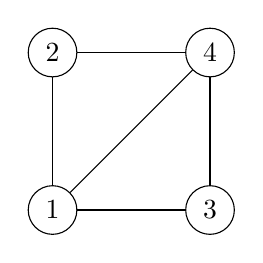
\begin{tikzpicture}
\node[circle,draw] (1) at (0,0){1};
\node[circle,draw] (2) at (0,2){2};
\node[circle,draw] (3) at (2,0){3};
\node[circle,draw] (4) at (2,2){4};
\foreach \from/\to in {1/2,1/3,1/4,2/4,3/4}
	\draw (\from)--(\to);
\end{tikzpicture}


\vspace{.5in}

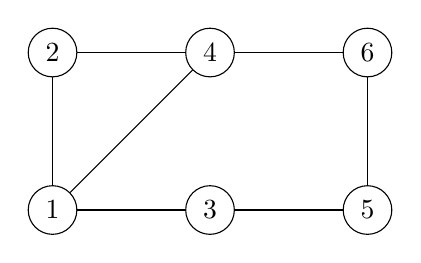
\begin{tikzpicture}
\node[circle,draw] (1) at (0,0){1};
\node[circle,draw] (2) at (0,2){2};
\node[circle,draw] (3) at (2,0){3};
\node[circle,draw] (4) at (2,2){4};
\node[circle,draw] (5) at (4,0){5};
\node[circle,draw] (6) at (4,2){6};
\foreach \from/\to in {1/2,1/3,1/4,2/4,4/6,6/5,3/5}
	\draw (\from)--(\to);
\end{tikzpicture}

\end{document}